% !TeX spellcheck = en_GB

\documentclass[a4paper,12pt]{article}

\usepackage{alltt, fancyvrb, url}
\usepackage{graphicx}
\usepackage{subfigure}
\usepackage{wrapfig}
\usepackage{algorithmic}
\usepackage[utf8]{inputenc}
\usepackage{fontenc}
\usepackage{amsmath,stmaryrd,mathtools,algorithm}
\usepackage{amssymb}
\usepackage{longtable}
\usepackage{multirow}
\usepackage{setspace}
\usepackage{todonotes}
\usepackage{csquotes}
\usepackage[margin=1.05in]{geometry}
\usepackage{todonotes}

% Remove option to use English naming
\usepackage[colorlinks,
	linkcolor={red!70!black},
	citecolor={blue!80!black},
	urlcolor={blue!50!black}]{hyperref}
\usepackage[nameinlink]{cleveref}

\usepackage{xcolor}
\usepackage{textcomp}
\usepackage{listings}


\definecolor{myPink}  {rgb}{0.67, 0.05, 0.57} % keywords
\definecolor{myRed}   {rgb}{0.87, 0.20, 0.00} % strings
\definecolor{myGreen} {rgb}{0.00, 0.47, 0.00} % comments
\definecolor{myBrown} {rgb}{0.39, 0.22, 0.13} % brown

\lstdefinestyle{Xcode} {
	language        = C,
	basicstyle      = \footnotesize\ttfamily,
	identifierstyle = \color{black},
	commentstyle    = \color{myGreen},
	keywordstyle    = \color{myPink},
	stringstyle     = \color{myRed},
	directivestyle  = \color{myBrown},
	extendedchars   = true,
	tabsize         = 4,
	showspaces      = false,
	showstringspaces = false,
	breakautoindent = true,
	flexiblecolumns = true,
	keepspaces      = true,
	stepnumber      = 1,
	xleftmargin     = 0pt,
	numbers=left
}

\lstset{
	style=Xcode,
	%caption=lstname,
	breaklines=false,
	frame=single
}

\title{Data visualization -- Process Book\\\textbf{Work in progress}}
\setcounter{tocdepth}{3}
\setcounter{secnumdepth}{3}
 
\author{Dario Pavllo \and Niccolò Sacchi \and Mattia Martinelli}
\date{} %\today

\begin{document}
\pagenumbering{arabic}
\maketitle
\section{Overview}
Buying from huge e-commerce websites such as \emph{Amazon} has many advantages, but, paradoxically, users are often confused by the vast variety of products. Users may have a rough idea about the characteristics of the product they want to buy, and they often undergo the same process of comparing similar products. We aim to remove this redundancy and aid them in their purchases, suggesting the best or most popular products that correspond to their search. For instance, comparing smartphones or laptops may be difficult due to the technical knowledge required, as well as the wide range of price covered. Our idea is to create a platform that allows a user to find the best product within a group of products with similar characteristics.

\subsection{Idea}
The idea is to exploit the relations in the Amazon product graph, such as ``bought together'', ``also viewed'', and/or ``buy after viewing''. These links reflect the behaviour of the users that buy on the famous e-commerce website, and can be used for providing recommendations to new or inexperienced users who want to purchase a certain kind of product.

At this point, a question naturally comes to mind: what is the added value to Amazon's website? It is true that these links can be found on Amazon, but they cannot offer a view ``as a whole''. From an article, a user can see the immediate neighbours, but that does not offer much information. On the contrary, if the user is presented with a visualization such as the one shown in \Cref{fig:graphNav}, it is very clear on which products users usually end up. In that example scenario, imagine that a user wants to buy some professional studio headphones, and has a rough idea of the characteristics of the product. By querying the graph, he/she can highlight relevant products and follow the path along the best product. Of course, \emph{best product} is relative; however, if many clients buy the same product after reviewing a set of other products, then it is very likely that the former has better characteristics.

\begin{figure}[H]
	\centering{}
	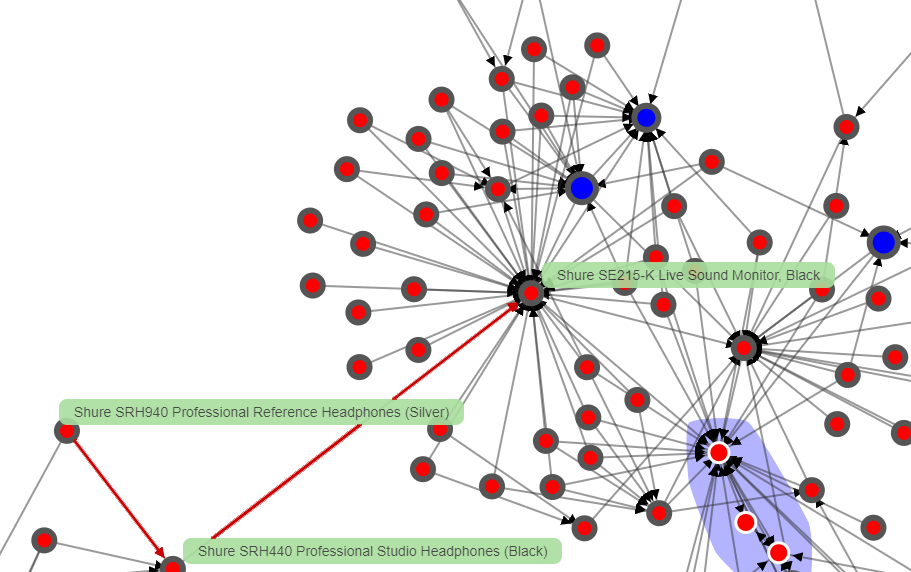
\includegraphics[width=\textwidth]{img/graph_nav.png}
	\caption{Subgraph of the \emph{Headphones} category. As can be seen, some nodes (products) are \emph{attractors}, in the sense that users end up buying those after reviewing a large number of other products.}
	\label{fig:graphNav}
\end{figure}

\section{The dataset}
We build groups of similar products using the \href{http://jmcauley.ucsd.edu/data/amazon/}. The dataset contains relations among products such as "bought together", "bought after viewing". These relations will be used for creating a graph that represents competing products with similar characteristics, i.e. products that are viewed together but not bought together. Our assumption is that people interested in a certain product would have visualized and compared similar products prior to buying whichever they consider the best.

\section{The graph}
At this stage, the graph is built by adding an edge between product A and product B if B is bought after viewing A. Conversely, if two products are frequently bought together, we remove the edge between them. In our context, a directed edge between A and B means ``B is better than A``, whereas an undirected edge (or, equivalently, two opposite directed edges) means ``A is competing with B''.

It is easy to extend this definition to groups of competing products, that is, max-cliques. If some groups are totally interconnected, we can assume that they are in direct competition and that one is not necessarily better than the other.

\section{Visualization}
The basic (and draft) idea of the visualization is to have guided navigation from the idea of the user to the final result. In particular, the process should be as follows:
\begin{enumerate}
	\item The user is presented with a selector that navigates through the Amazon category tree, and allows him/her to select a category (e.g. headphones, mobile phones, laptops, etc.) Of course, it will also be possible to search for a category according to some keywords.
	\item Once a category is selected, the graph view appears. Initially, the full graph is shown, so that the user can get a sense of its topology (sparseness, attractors, cliques, etc.).
	\item The user can query a few keywords and set a price range, which will cause the graph to highlight only relevant parts and collapse the rest. At this point, the user can inspect the paths between products, as well as the \emph{attractors}. The visualization will also provide some recommendations (automatic paths) and display the characteristics of the products, along with their differences.
\end{enumerate}


\end{document}